% ============================================================================
% Tests report: the three filmed tests, files, analysis settings and time base.
% ============================================================================
\section{Ensayos y datos}\label{sec:videos}

\subsection{Los ensayos}

Se analizaron tres ensayos con 22 robots en la misma arena circular y el mismo modo de movimiento
(\texttt{QR}), filmados con una cámara DJI fija sobre la arena, mirando hacia abajo (\cref{tab:ensayos}). Se identifican por fecha y
hora de inicio; en tablas y gráficos se usan las etiquetas \Cmp{Lab}{A}, \Cmp{Lab}{B} y \Cmp{Lab}{C}.
El recinto tiene un diámetro interior de \SI{\DiametroIntRecintoCM}{\centi\metre}
($R_{\mathrm{int}} = \SI{\Cmp{Rar}{A}}{\centi\metre}$), de modo que los robots
(\SI{\DiametroRobotCM}{\centi\metre} de diámetro) cubren una fracción de área
$\phi = N(D/2)^2/R_{\mathrm{int}}^2 = \num{\Cmp{Phi}{A}}$: es un sistema denso, en el que cada robot está
casi siempre en contacto con sus vecinos. (Hasta el 07/10 se informaba $\phi \approx 0{,}58$, calculado con
una escala errónea y un radio deducido de las trayectorias; ver \cref{sec:recinto_ens}.)

\begin{table}[H]
  \centering
  \caption{Ensayos analizados. Duración real con $\fr = \num{\CuadrosPorSegundo}$~cuadros/s.}
  \label{tab:ensayos}
  \small
  \begin{tabular}{@{}llrrr@{}}
    \toprule
    Etiqueta & Código & Cuadros (\texttt{VC}) & Duración real & Recorte [px] \\
    \midrule
    \Cmp{Lab}{A} & \texttt{20262409\_1600\_22QR\_60} & \num{12069} & \SI{67.0}{\minute} & $610\times610$ \\
    \Cmp{Lab}{B} & \texttt{20262509\_1230\_22QR\_60} & \num{9881}  & \SI{54.9}{\minute} & $610\times614$ \\
    \Cmp{Lab}{C} & \texttt{20262509\_1500\_22QR\_60} & \num{11012} & \SI{61.2}{\minute} & $604\times614$ \\
    \bottomrule
  \end{tabular}
\end{table}

\subsection{Archivos}

Cada ensayo tiene, con el mismo \texttt{<código>}, los archivos de la \cref{tab:archivos_ens}. El
código es: fecha (año, día, mes: \texttt{20262409} = 24/09/2026), hora de inicio, cantidad de robots
y modo, y duración \emph{nominal} en minutos (la medida difiere, ver \cref{sec:escala_ens}).

\begin{table}[H]
  \centering
  \caption{Archivos de cada ensayo.}
  \label{tab:archivos_ens}
  \small
  \begin{tabular}{@{}p{6.0cm}p{8.6cm}@{}}
    \toprule
    Archivo & Contenido \\
    \midrule
    \nolinkurl{datos/video/originales/VR_<codigo>.MP4} & original de la cámara, \num{3840}\,$\times$\,\num{2160}\,px, H.264, \SI{29.97}{cuadros\per\second} \\
    \nolinkurl{datos/video/recortados/VC_<codigo>.MP4} & recorte a la arena (unos \num{610}\,$\times$\,\num{610}\,px); empieza al terminar el pulso LED de sincronización (\cref{sec:escala_ens}) \\
    \nolinkurl{datos/video/sesiones/VA_<codigo>_analisis.npz} & sesión de análisis de VidFetch (candidatos, firmas, anclas, parámetros) \\
    \nolinkurl{datos/video/trayectorias/VP_<codigo>_robots.csv} & datos exportados: una fila por robot y cuadro (origen en el centro del recinto) \\
    \nolinkurl{datos/video/trayectorias/VP_<codigo>_robots_info.json} & recinto, escala y convenciones de ese CSV \\
    \nolinkurl{datos/video/trayectorias/VP_<codigo>_robots_resumen.csv} & una fila por robot (rapidez, giro, capa de la pared\ldots) \\
    \nolinkurl{datos/presion/crudos/R_<codigo>.csv} & registro del sensor de presión (FSR), \SI{20}{\hertz}, con columna \texttt{LED} de sincronización \\
    \bottomrule
  \end{tabular}
\end{table}

\subsection{Configuración del análisis}

Los tres videos se analizaron con VidFetch con la calibración automática, que dio parámetros casi
idénticos (\cref{tab:config}), lo que confirma que la cámara estuvo a la misma altura y con la misma
iluminación. El método está descripto en el informe de la aplicación.

\begin{table}[H]
  \centering
  \caption{Parámetros usados (guardados en cada sesión \texttt{VA\_*.npz}).}
  \label{tab:config}
  \small
  \begin{tabular}{@{}lrrr@{}}
    \toprule
    Parámetro & \Cmp{Lab}{A} & \Cmp{Lab}{B} & \Cmp{Lab}{C} \\
    \midrule
    Radio exterior del robot $r_{\mathrm{ext}}$ [px] & \num{47.0} & \num{47.0} & \num{47.1} \\
    Radio del disco $r_{\mathrm{int}}$ [px] & \num{35.2} & \num{35.3} & \num{35.3} \\
    Escala espacial (recinto, mediana) [\si{\milli\metre\per px}] & \num{\Cmp{Esc}{A}} & \num{\Cmp{Esc}{B}} & \num{\Cmp{Esc}{C}} \\
    Diámetros del recinto / del robot & \multicolumn{3}{c}{\SI{185}{} y \SI{195}{\milli\metre} / \SI{33}{\milli\metre}} \\
    Medición del recinto & \multicolumn{3}{c}{cada \Cuadros{30}, mediana móvil de 5 muestras} \\
    Gris máximo del anillo / del píxel oscuro & 106 / 68 & 111 / 71 & 104 / 68 \\
    Cobertura mínima del anillo & \multicolumn{3}{c}{\num{0.82} (relajada: \num{0.70} y \num{0.55})} \\
    Radio de búsqueda [px] & \multicolumn{3}{c}{\num{29.4} ($0{,}625\,r_{\mathrm{ext}}$)} \\
    Ventana de Savitzky--Golay & \multicolumn{3}{c}{\Cuadros{5}, polinomio de grado 2} \\
    Escala de tiempo $\fr$ & \multicolumn{3}{c}{\num{3} cuadros por segundo real} \\
    Orientación de la escena & \multicolumn{3}{c}{imagen rotada \SI{180}{\degree} (vista del observador; no espejada)} \\
    \bottomrule
  \end{tabular}
\end{table}

\subsection{El recinto: origen, escala y movimiento}\label{sec:recinto_ens}

Todas las posiciones de este informe tienen origen en el centro del recinto y están en el sistema de la
vista del observador: quien hizo los ensayos estaba parado del lado del borde superior del video
($y_{\mathrm{px}} = 0$), mirando hacia el inferior ($y_{\mathrm{px}} = 2160$ en el video original). Las
imágenes se muestran rotadas \SI{180}{\degree} para verlas desde ahí: $x$ queda a la derecha del
observador (la izquierda del video original), $y$ hacia la pared de enfrente y los ángulos son positivos en
sentido antihorario visto desde arriba. Una rotación no cambia el sentido de giro, a diferencia de un
espejado. Las posiciones están en milímetros con la escala que da el diámetro interior del
recinto, $D_{\mathrm{int}} = \SI{185}{\milli\metre}$ (método en el informe de la aplicación). El recinto
se midió cada \num{30}~cuadros (\SI{10}{\second}) en los tres videos (\cref{tab:recinto}).

\begin{table}[H]
  \centering
  \caption{Recinto medido en cada ensayo. Escala y radios: medianas sobre el ensayo.}
  \label{tab:recinto}
  \small
  \begin{tabular}{@{}lrrr@{}}
    \toprule
    & \Cmp{Lab}{A} & \Cmp{Lab}{B} & \Cmp{Lab}{C} \\
    \midrule
    Radio interior en la imagen [px] & \num{286.1} & \num{285.4} & \num{286.4} \\
    Escala $s = (D_{\mathrm{int}}/2)/r_{\mathrm{int}}$ [\si{\milli\metre\per px}] & \num{\Cmp{Esc}{A}} & \num{\Cmp{Esc}{B}} & \num{\Cmp{Esc}{C}} \\
    $r_{\mathrm{ext}}/r_{\mathrm{int}}$ medido (esperado \num{1.0541}) & \num{1.0545} & \num{1.0547} & \num{1.0547} \\
    Residuo del borde interior [px] & \num{\Cmp{ResR}{A}} & \num{\Cmp{ResR}{B}} & \num{\Cmp{ResR}{C}} \\
    Desplazamiento del recinto en $x$ / $y$ [\si{\milli\metre}] & \Cmp{MovX}{A} / \Cmp{MovY}{A} & \Cmp{MovX}{B} / \Cmp{MovY}{B} & \Cmp{MovX}{C} / \Cmp{MovY}{C} \\
    Variación de escala (zoom de la cámara) [\si{\percent}] & \num{\Cmp{Zoom}{A}} & \num{\Cmp{Zoom}{B}} & \num{\Cmp{Zoom}{C}} \\
    Radio de contacto $R_{\mathrm{c}} = q_{99.5}(r)$ [\si{\milli\metre}] & \num{\Cmp{Rc}{A}} & \num{\Cmp{Rc}{B}} & \num{\Cmp{Rc}{C}} \\
    Factor de perspectiva $\kappa = (R_{\mathrm{int}} - D/2)/R_{\mathrm{c}}$ & \num{\Cmp{Kap}{A}} & \num{\Cmp{Kap}{B}} & \num{\Cmp{Kap}{C}} \\
    \bottomrule
  \end{tabular}
\end{table}

\paragraph{El recinto se mueve y la cámara cambia de aumento.} El centro del recinto no está fijo en la
imagen (\cref{fig:recinto_mov}). En los tres ensayos sigue el mismo patrón: durante los primeros
\SI{15}{\minute} se aleja unos \SI{2}{\milli\metre} del observador ($+y$) y entre los minutos 15 y 30
vuelve, con oscilaciones de
$\pm\SI{1}{\milli\metre}$ en $x$ al comienzo; después queda quieto dentro de $\pm\SI{0.5}{\milli\metre}$.
La placa de fondo, en cambio, no se mueve (correlación de fase de las esquinas del cuadro: corrimiento
constante menor que \SI{1}{px}), así que es el anillo el que se desliza sobre la placa, probablemente
empujado por los robots y la vibración. Además, el radio aparente salta \SI{0.5}{\percent} de golpe
(24/09 en el minuto 18, 25/09 15:00 en el minuto 13; 25/09 12:30 empieza ya en el valor alto). En ese
salto la placa de fondo también se agranda \SI{0.47}{\percent}, de modo que es un cambio de aumento de
la cámara (reenfoque) y no del anillo. Las dos cosas se corrigen midiendo el recinto a lo largo del
video: cada posición se refiere al centro y a la escala de su propio cuadro. Con un único centro fijo,
las posiciones tendrían errores de hasta \SI{4}{\milli\metre} y las capas de la \cref{fig:cmp_ocupacion}
saldrían borroneadas.

\begin{figure}[H]
  \centering
  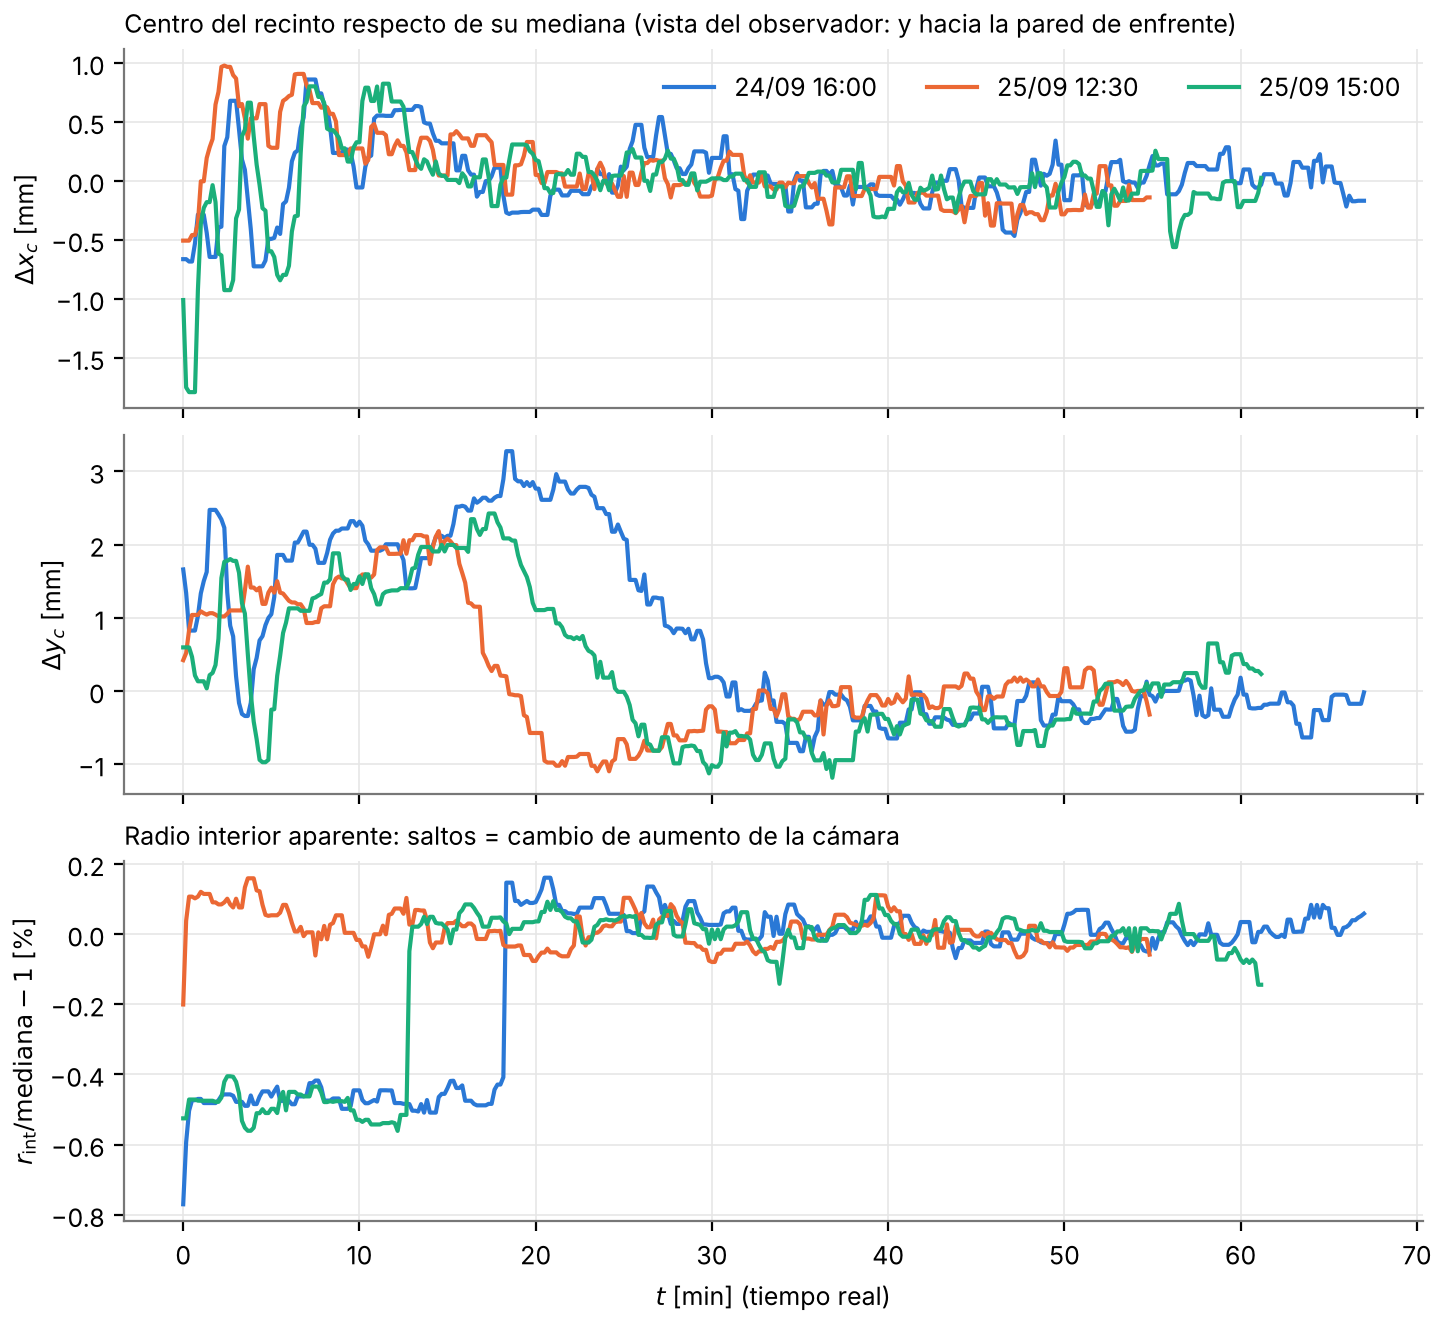
\includegraphics[width=0.95\linewidth]{figuras/recinto_movimiento.png}
  \caption{Centro del recinto (respecto de su mediana, en el sistema de la vista del observador) y radio aparente a lo largo de cada
    ensayo, después de la mediana móvil de 5 muestras. Los saltos del radio coinciden con un agrandamiento
    igual de la placa de fondo: son cambios de aumento de la cámara.}
  \label{fig:recinto_mov}
\end{figure}

\paragraph{La escala es consistente por tres caminos independientes.}
\begin{enumerate}
  \item El cociente de los radios exterior e interior del anillo, que no depende de la escala, coincide
        con $D_{\mathrm{ext}}/D_{\mathrm{int}} = 195/185$ con \SI{0.05}{\percent} (\cref{tab:recinto}).
  \item El cuerpo de los robots (borde de la placa, con LEDs y componentes) mide \SI{101}{px} de
        diámetro en la imagen (mediana sobre \num{4870} rayos sin vecinos en 21 cuadros de \Cmp{Lab}{A};
        rango intercuartil \num{99}--\SI{107}{px}): con $s = \SI{0.323}{\milli\metre\per px}$ son
        \SI{32.7}{\milli\metre}, el diámetro real.
  \item La capa de la pared y la capa media están a \SI{75.2}{} y \SI{42.8}{\milli\metre} del centro en los
        tres ensayos: separadas \SI{32.5}{\milli\metre}, prácticamente un diámetro de robot, como
        corresponde a discos densos apoyados unos en otros.
\end{enumerate}
La escala usada hasta el 07/10 ($s = D/(2\,r_{\mathrm{ext}}) = \SI{0.372}{\milli\metre\per px}$, con
$D = \SI{35}{\milli\metre}$ y el radio del anillo oscuro que usa el detector, $r_{\mathrm{ext}} = \SI{47}{px}$)
no cumple ninguna de las tres: haría que el recinto midiera \SI{213}{\milli\metre} de diámetro y que las
capas estuvieran separadas \SI{37.4}{\milli\metre}, más que un robot. El anillo oscuro es más chico que
el cuerpo del robot. Por eso \textbf{todas las longitudes y velocidades de este informe son
\SI{13}{\percent} menores que en la versión anterior} (factor $0{,}3233/0{,}372 = \num{0.869}$); los
ángulos, $\omega$, los tiempos y los estados de seguimiento no cambian.

\paragraph{Perspectiva.} Los robots apoyados en la pared tienen su centro a $R_{\mathrm{c}} \approx
\SI{78}{\milli\metre}$ del centro, mientras que con $D = \SI{33}{\milli\metre}$ deberían estar a
$R_{\mathrm{int}} - D/2 = \SI{76}{\milli\metre}$. La diferencia (\SI{2.5}{\percent}) es de perspectiva: la
cámara mide el centro del robot en su parte superior y el radio del recinto en el canto del anillo, a
alturas distintas. Se deja sin corregir ($\kappa$ no se aplica) y se toma como incertidumbre sistemática
de las posiciones y velocidades; la aplicación permite aplicarla (\emph{Escala desde: recinto + corrección
de perspectiva}).

\subsection{Escala de tiempo y sincronización con el sensor}\label{sec:escala_ens}

Los videos son \emph{time-lapse}: cada cuadro se toma cada $1/\fr$ segundos reales y el archivo se
reproduce a \SI{29.97}{cuadros\per\second}, unas 10 veces más rápido. Todos los tiempos, velocidades
y velocidades angulares de este informe están en tiempo real con $\fr = 3$~cuadros/s. El valor se
verificó de tres maneras independientes:
\begin{enumerate}
  \item \textbf{Configuración de la cámara}: un \emph{time-lapse} $\times 10$ a \SI{29.97}{cuadros\per\second}
        da $\fr = \num{2.997}$.
  \item \textbf{Duración del registro del sensor}, grabado en simultáneo con su propio reloj
        (\cref{tab:videos}).
  \item \textbf{Correlación con el sensor}: al barrer $\fr$ entre \num{2.985} y \num{3.015}, la correlación
        entre la movilidad de los robots y la señal del sensor es máxima entre \num{2.9975} y \num{3.0025}
        en los tres ensayos (\cref{sec:presion}).
\end{enumerate}
La duración nominal del nombre (\SI{60}{\minute}) \emph{no} sirve para calcular $\fr$: daría valores
entre \num{2.75} y \num{3.36}, con errores de hasta \SI{12}{\percent} en todas las velocidades.

\begin{table}[H]
  \centering
  \caption{Cuadros de los originales (\texttt{VR}) y frecuencia de captura deducida de tres maneras.
    Duración del sensor: $t_{\text{último}} - t_{\text{primero}}$ de \texttt{R\_<código>.csv}; como el
    registro empieza antes que el video, el $\fr$ que da es una cota inferior.}
  \label{tab:videos}
  \small
  \begin{tabular}{@{}lrrrrrr@{}}
    \toprule
    & & \multicolumn{2}{c}{$T$ con $\fr = \num{2.997}$} & \multicolumn{2}{c}{Sensor de presión} & Nominal \\
    \cmidrule(lr){3-4}\cmidrule(lr){5-6}\cmidrule(l){7-7}
    Ensayo & Cuadros & video [\si{\second}] & real [\si{\minute}] & $T$ [\si{\second}] & $\fr$ & $\fr$ (\SI{60}{\minute}) \\
    \midrule
    \Cmp{Lab}{A} & \num{12105} & \num{403.9} & \num{67.3} & \num{4055.1} & \num{2.985} & \num{3.36} \\
    \Cmp{Lab}{B} & \num{9907}  & \num{330.6} & \num{55.1} & \num{3368.4} & \num{2.941} & \num{2.75} \\
    \Cmp{Lab}{C} & \num{11038} & \num{368.3} & \num{61.4} & \num{3699.5} & \num{2.984} & \num{3.07} \\
    \bottomrule
  \end{tabular}
\end{table}

\paragraph{Sincronización.} El registrador del sensor enciende un LED durante \SI{5}{\second} al
comenzar (columna \texttt{LED}). En los tres ensayos, el primer cuadro del video recortado
(\texttt{VC}) coincide con el \emph{fin} de ese pulso: la correlación cruzada entre video y sensor,
calculada sin usar el LED, da el mismo desfasaje con diferencias de \SI{\Cmp{LagLed}{A}}{\second},
\SI{\Cmp{LagLed}{B}}{\second} y \SI{\Cmp{LagLed}{C}}{\second}, menores que dos cuadros. Por lo tanto,
el tiempo del sensor se pasa al del video con
\begin{equation}
  t_{\mathrm{video}} = t_{\mathrm{sensor}} - t_{\mathrm{LED,fin}},
\end{equation}
con $t_{\mathrm{LED,fin}}$ = \SI{\Cmp{LedFin}{A}}{\second}, \SI{\Cmp{LedFin}{B}}{\second} y
\SI{\Cmp{LedFin}{C}}{\second} desde el inicio de cada registro.
